\documentclass{beamer}
\usetheme{metropolis}
\usepackage{graphicx}
\usepackage{subfig}
\usepackage{hyperref}
\usepackage{tcolorbox}
\title{Algebra-Based Physics-1: Mechanics (PHYS135A-01): Week 6}
\date{October 9th - October 13th, 2017}
\author{Jordan Hanson}
\institute{Whittier College Department of Physics and Astronomy}

\begin{document}
\maketitle

\section{Week 5 Review}

\begin{frame}{Week 5 Review}
\begin{enumerate}
\item \alert{Friction}
\begin{itemize}
\item Normal force and friction
\item Static, kinetic
\end{itemize}
\item \alert{Drag}
\begin{itemize}
\item Terminal velocity
\end{itemize}
\item \alert{Restoring Forces}
\begin{itemize}
\item Hooke's Law
\item Young's modulus
\item Shear modulus
\item Bulk modulus
\end{itemize}
\end{enumerate}
\end{frame}

\section{Week 5 Review Problem}

\begin{frame}{Week 5 Review Problem}
A car rests on four shock absorbers, and each is like a spring with a spring constant $k = 1000 N/cm$.  The car weighs 10000 N.  By what distance is each spring compressed?
\begin{itemize}
\item A: 2.5 cm
\item B: 10 cm
\item C: 1 meter
\item D: 0 cm
\end{itemize}
\end{frame}

\begin{frame}{Week 5 Review Problem}
A team of workers is pulling a 500 kg load up a ramp with a 30 degree incline, at constant speed, and the coefficient of friction between the load and ramp is 0.6.  What is the force with which the workers pull?
\begin{itemize}
\item A: 5000 N
\item B: 2500 N
\item C: 2750 N
\item D: 3750 N
\end{itemize}
\end{frame}

\section{Week 6 Summary}

\begin{frame}{Week 6 Summary}
\begin{enumerate}
\item \alert{Angular} kinematics
\begin{itemize}
\item Angular displacement
\item Angular velocity
\item centripetal acceleration
\end{itemize}
\item \alert{Newton's Law of Gravity} and circular orbits
\item Kepler's Laws
\end{enumerate}
\end{frame}

\section{Angular Kinematics}

\begin{frame}{Angular Kinematics}
There is a correspondence between \alert{angular and linear kinetmatics}, if we deal with accelerations that are constant or zero.
\begin{columns}[T]
\begin{column}{0.5\textwidth}
\centering
\textbf{Linear}:
\begin{align}
x(t) &= x_{\rm 0} + v_{\rm i}t + \frac{1}{2}at^2 \\
v(t) &= v_{\rm i}t + at \\
v^2 &= v_{\rm i}^2 + 2a(x-x_{\rm 0})
\end{align}
\end{column}
\begin{column}{0.5\textwidth}
\centering
\textbf{Angular}:
\begin{align}
\theta(t) &= \theta_{\rm 0} + \omega_{\rm i}t + \frac{1}{2}\alpha t^2 \\
\omega(t) &= \omega_{\rm i}t + \alpha t \\
\omega^2 &= \omega_{\rm i}^2 + 2\alpha\Delta(\theta-\theta_{\rm 0})
\end{align}
\end{column}
\end{columns}
\end{frame}

\begin{frame}{Angular Kinematics}
\begin{figure}
\centering
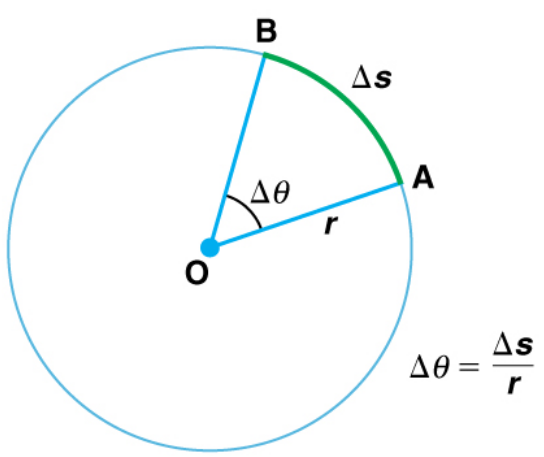
\includegraphics[width=0.6\textwidth]{figures/circle1.png}
\caption{\label{fig:circle1} The definitions of arc length, $\Delta s$, radius, r, and angular displacement $\Delta\theta$.}
\end{figure}
\end{frame}

\begin{frame}{Angular Kinematics}
\begin{columns}[T]
\begin{column}{0.5\textwidth}
\begin{figure}
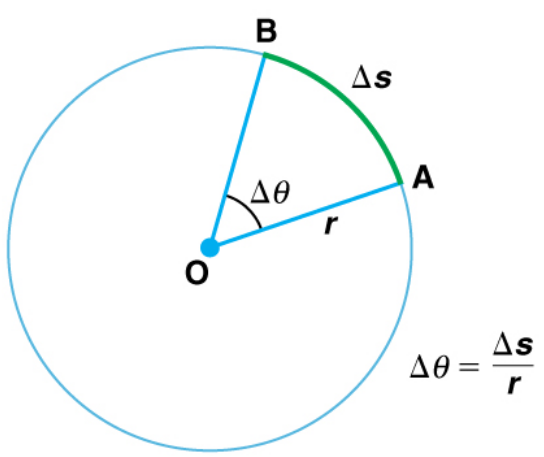
\includegraphics[width=0.6\textwidth]{figures/circle1.png}
\caption{\label{fig:circle2} \small Examining the change in these quantities: $\Delta\theta/\Delta t = \omega$, $\Delta\omega/\Delta t = \alpha$.}
\end{figure}
\end{column}
\begin{column}{0.5\textwidth}
\centering
Relationship between linear and rotational:
\begin{align}
v = \frac{\Delta s}{\Delta t} &= r \frac{\Delta\theta}{\Delta t} = r\omega \\
a = \frac{\Delta v}{\Delta t} &= r \frac{\Delta\omega}{\Delta t} = r\alpha
\end{align}
Notice that the units of angular velocity are s$^{-1}$, and those of angular acceleration are s$^{-2}$.
\end{column}
\end{columns}
\end{frame}

\begin{frame}{Angular Kinematics}
Astromers have now discovered several thousand planets orbiting in star systems other than ours.  Suppose we observe a star system face-on, and see a planet orbiting in a circular orbit with constant angular velocity.  If it goes halfway around the star in 3 months, what is the angular velocity of the planet?
\begin{itemize}
\item A: $\frac{\pi}{3}$ months$^{-1}$
\item B: $\frac{\pi}{6}$ months$^{-1}$
\item C: $\frac{2\pi}{3}$ months$^{-1}$
\item D: $2\pi$ months$^{-1}$
\end{itemize}
\end{frame}

\begin{frame}{Angular Kinematics}
If we define a coordinate system such that at time $t = 0$ months, the planet is along the x-axis, in how many months will the planet cross the negative y-axis?
\begin{itemize}
\item A: 3 months
\item B: 3.5 months
\item C: 4.0 months
\item D: 4.5 months
\end{itemize}
\end{frame}

\begin{frame}{Angular Kinematics}
\begin{columns}[T]
\begin{column}{0.5\textwidth}
\begin{figure}
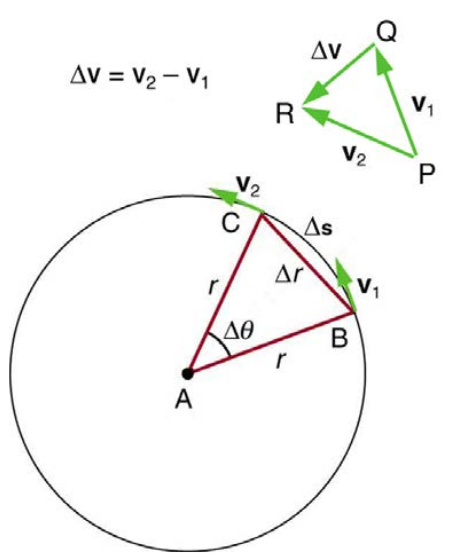
\includegraphics[width=0.6\textwidth]{figures/circle2.png}
\caption{\label{fig:circle3} \small The velocity triangle and the position triangle are \textit{similar}, because they are isosceles with the same angle ($\Delta\theta$).}
\end{figure}
\end{column}
\begin{column}{0.5\textwidth}
\centering
Similar triangles have equal \textit{ratios of sides}:
\begin{align}
\frac{\Delta v}{v} &= \frac{\Delta s}{r} \\
\Delta v &= \frac{v}{r}\Delta s \\
\frac{\Delta v}{\Delta t} &= \frac{v}{r}\frac{\Delta s}{\Delta t} \\
\Delta t &\to 0 \\
a_{\rm C} &= \frac{v^2}{r} = r \omega^2 \\
\vec{a}_{\rm C} &= - \frac{v^2}{r} \hat{r}
\end{align}
\end{column}
\end{columns}
\end{frame}

\begin{frame}{Angular Kinematics}
With centripetal acceleration comes \textbf{\alert{centripetal force}}, which is the net force for uniform circular motion:
\begin{equation}
\vec{F}_{\rm C} = - \frac{mv^2}{r}\hat{r} = -m r \omega^2 \hat{r}
\label{eq:centripetalForce}
\end{equation}
In Eq. \ref{eq:centripetalForce}, the minus sign indicates that the force points towards the center of the circle.
\end{frame}

\begin{frame}{Angular Kinematics}
Example problem with centripetal acceleration and force.
\begin{itemize}
\item A: 5000 N
\item B: 2500 N
\item C: 2750 N
\item D: 3750 N
\end{itemize}
\end{frame}

\section{Conclusion}

\begin{frame}{Week 6 Summary}
\begin{enumerate}
\item \alert{Angular} kinematics
\begin{itemize}
\item Angular displacement
\item Angular velocity
\item centripetal acceleration
\end{itemize}
\item \alert{Newton's Law of Gravity} and circular orbits
\item Kepler's Laws
\end{enumerate}
\end{frame}

\section{Answers}

\begin{frame}{Answers}
\begin{columns}[T]
\begin{column}{0.5\textwidth}
\begin{itemize}
\item 2.5 cm
\item 2750 N
\item $\frac{\pi}{3}$ months$^{-1}$
\item 4.5 months
\end{itemize}
\end{column}
\begin{column}{0.5\textwidth}
\begin{itemize}
\item ... 
\end{itemize}
\end{column}
\end{columns}
\end{frame}

\end{document}
